\documentclass{article}
\usepackage[english]{babel}
\usepackage[utf8]{inputenc}
\usepackage[margin=1.5in]{geometry}
\usepackage{amsmath}
\usepackage{amsthm}
\usepackage{amsfonts}
\usepackage{amssymb}
\usepackage[usenames,dvipsnames]{xcolor}
\usepackage{graphicx}
\usepackage{multicol}
\usepackage[siunitx]{circuitikz}
\usepackage{tikz}
\usepackage[colorinlistoftodos, color=orange!50]{todonotes}
\usepackage{hyperref}
\usepackage[numbers, square]{natbib}
\usepackage{fancybox}
\usepackage{epsfig}
\usepackage{soul}
\usepackage[framemethod=tikz]{mdframed}

\usepackage{fancyhdr}
\pagestyle{fancy}
\fancyhf{}
\lhead{Darshan Patel}
\rhead{Big Data Programming Course Project}
\renewcommand{\footrulewidth}{0.4pt}
\cfoot{\thepage}


\setlength{\marginparwidth}{3.4cm}

\setlength\parindent{0pt}

\title{
\normalfont \normalsize 
\textsc{Fordham University New York, NY \\ 
Big Data Programming, Fall 2018} \\
[10pt] 
\rule{\linewidth}{0.35pt} \\[12pt] 
\LARGE Data Analysis of Citi Bikes from January - October 2018 
\rule{\linewidth}{2pt}  \\[10pt]
}
\author{Darshan Patel \\~\\ Professor Yijun Zhao}
\date{\normalsize \today}

\begin{document}

\maketitle
\noindent
%Date Performed \dotfill January 0, 0000 \\
%Partners \dotfill Full Name \\
%Instructor \dotfill Full Name \\
\tableofcontents

\newpage
\section{Abstract}
New York City is known to have one of the largest train system in the world. However it is not the best or most reliable solution for transportation at times. Looking at other options include driving by personal vehicle, Uber, walking and bicycling. Bicycling is a widely used mode of transportation in NYC thanks to the launch of Citi bikes by Citi Bank. In this project, a variety of big data technologies such as Spark, Spark RDD and Spark SQL were used to answer interesting questions about millions of Citi bikers. These questions are: 
\begin{itemize} 
\item What are the top 5 destinations for Citi bikers based on departure time? Which areas are popular? 
\item What is the distribution of user types per age? 
\item What is the distribution of bike uses depending on the time of day, type of day and gender? 
\item What are the most common bikes used? What are the total hours they are used? 
\item What is the average distance traveled by age and gender? Their average Speed? 
\end{itemize} 
These are just some of the many questions that can be derived from looking at this dataset. In addition, a linear regression model was also made, using the MLlib package, that predicted the duration of a trip based on the distance between the stations calculated using the Haversine formula for great-circle distance between two points. 

\newpage

\section{Dataset} 
The Citi bike trip dataset is composed of several columns of data: 
\begin{multicols}{2} \begin{itemize} 
\item Trip duration (seconds)
\item Start Time and Date
\item Stop Time and Date
\item Start Station Name and ID
\item Start Station Latitude and Longitude Coordinates 
\item End Station Name and ID
\item End Station Latitude and Longitude Coordinates 
\item Bike ID
\item User Type 
\item Gender 
\item Year of Birth \end{itemize} \end{multicols} 
Most of these features are self-explanatory. For each observation, various trip information was noted. The starting and ending point of each trip was noted, including the station name, station ID and the coordinates of the station itself. The duration of the trip was jotted down in seconds as well as the individual ID number of the bike in use. About the biker, their user type, gender and year of birth was noted. The user type feature is grouped into two categories: customers and subscribers. Customers of Citi bikes are people who either brought a $24$ hour pass or a $3$ day pass; meaning they are only temporary users. On the other hand, subscribers of Citi bikes are people who hold an annual membership. 

Citi Bike publishes their data in terms of month and location. Meaning, one document is for bike uses in NYC while the other is for Jersey City. For this project, only the data that pertains to NYC will be used. In addition, data from 2018 only was used. At the time when the project was started, data up to October was published. These $10$ datasets, together, was of size $2.83$ gigabytes in csv format. When attempting to open one of these files in Microsoft Excel, the program lagged due to the size of the file. In addition, it reported that some features might be lost. Using ordinary data analysis tools did not seem to be a good idea here and so Spark RDD was the next option. 

After downloading each individual dataset for each month, each monthly data file was uploaded to Spark as a resilient distributed dataset (RDD). The ten RDDs were put together to create a single RDD that stored all the Citi bike data from the year of 2018. In total, this made a total number of observations to be $15,271,479$. Good thing Spark can handle this easily. 

\newpage
\section{Data Cleaning}
Before starting to analyze the data, it is important to eliminate any possible noise that is in the data. After researching about the Citi bike membership and the actual data file, it appeared that there were several features that needed to be cleaned. Firstly, it was found that in the original dataset, the gender column was filled with three genders: male, female and unknown, the following distribution 
$$ \begin{tabular}{|c|c|} \hline Gender & Count \\ \hline Male & $0.675$ \\ Female & $0.234$ \\ Unknown & $0.089$ \\ \hline \end{tabular} $$ 
The unknown gender count made up for $8\%$ of the data while the male count was nearly three times as big as the female count. To clean this column, any records that had an unknown gender was filtered out. \\~\\
Next, the birth year column was analyzed. After changing the column to represent current age, it was found that there were many bikers who were $80+$ years old, as well as bikers who were up to $133$ years old. This cannot be true since the oldest verified living people in the world are in their $110$s and reside in other counties. In addition, their health is likely at a low quality and thus not ready to board an airplane to NYC so they can ride a Citi bike in Manhattan. It was found that the huge declination in bikers by age started at the age of $63$ years old. This is around the time that people start retiring from their job and become less able to be highly active. 
So for this study, people who are older than $65$ are filtered out. \\~\\
Another column that was to be questioned was the duration column with attention to the user type column. According to the Citi bike membership website, a $24$ hour pass and a $3$ day pass has a limit of $30$ mins of usage before they are charged again. In addition, annual members are also charged again when going over $45$ minutes. This feature was important to look at because there were countless observations that stated a trip lasted at least a thousand hours, or at least $10$ days. With the fact that bikers are charged for going above $30$ or $45$ minutes, it can be seen that trips that lasted too long were noisy data. Therefore, all trips that were longer than $30$ minutes for customer and $45$ minutes for a subscriber were filtered out. This may not be the most correct cut off point. Some people may have been open to being charged once or twice again; therefore it is debatable. \\~\\
The last columns that were investigated were the start and end station names. It was found several people made round trips on their Citi Bikes. This means that any analysis that had to do with distance traveled would be inaccurate, since the distance found would be $0$. Therefore any observations where the start and end station name was the same was also filtered. \\~\\
A lot of columns were cleaned during this process. But in actuality, not a lot of data was removed. This new reduced dataset has $13,189,622$ observations, which is only a $10.6\%$ decrease in size. This is still big data. 

\newpage
\section{Top $5$ destinations based on time of departure} 
The first question that was answered was, what are the top $5$ destinations bikers are going to based on the time of departure. Four different time slots were studied: morning, afternoon, night, and late night. \\~\\
For the morning bikers, from $5$AM to $12$PM, these were the most common destination stations. 
$$ 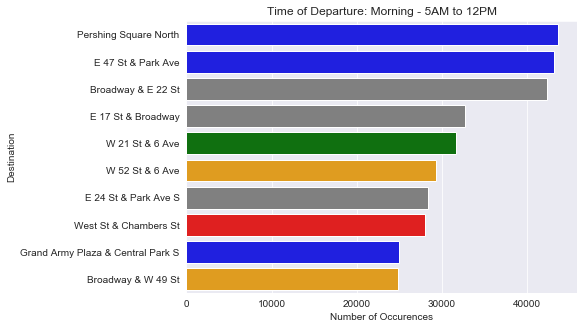
\includegraphics[scale = 0.6]{morningData} $$ 
The bars are colored by neighborhood such that: 
\begin{itemize} \item Orange represents Midtown West \item Blue represents Midtown East \item Red represents Lower Manhattan \item Grey represents Flatiron \item Green represents Chelsea \item Brown represents East Village \item Purple represents West Village \end{itemize} 
According to this bar graph, it can be seen that Pershing Square North,and E 47 St \& Park Avenue were two of the most common destinations for bikers in the morning. This makes sense since both are located in Midtown East. This area is populated by many financial firms and other businesses. Pershing Square North is actually the public square in Manhattan right in front of Grand Central Terminal. This is a heavy populated area, at any hour, at a matter of fact. In addition to Midtown East, three Flatiron stations were also popular in the morning. The three top most destinations traveled to had an occurrence of at least $40,000$ which the next most traveled to destination was slightly over $30,000$. \\~\\
For the afternoon bikers from noon to $6$ PM, these were the most common destination stations: 
$$ 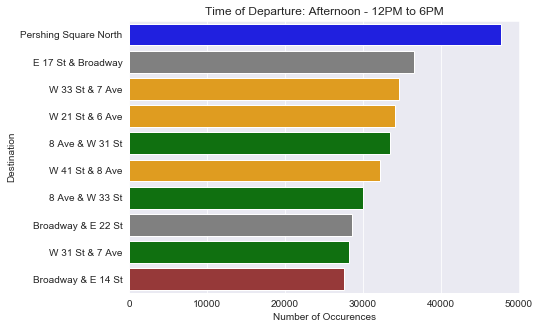
\includegraphics[scale = 0.6]{afternoonData} $$ 
The color code is the same as above and will remain as so below. In this bar graph, it is seen that there is only $1$ popular Midtown East destination, Pershing Square North. It has an occurrence of nearly $50,000$. This can be attributed to people who are traveling to the train station at this hour after work ended or people wanting to come to this area for shopping. The next most popular station barely touches $40,000$ trips. The third most popular stations in this time frame is East 17th Street and Broadway. This is a station that is near multiple train stations like Penn Station and Herald Square train station which people might be going to. The tenth most popular destination is Broadway and East 14th Street. This is located in the heart of Union Square, which is known to be a popular place of travel for tourists, as well as a small college ``town." Students may be traveling to here to attend classes at NYU, Cooper Union, Cardozo School of Law, Yeshiva University, etc.  \\~\\
For the evening bikers from $6$PM to $10$PM: 
$$ 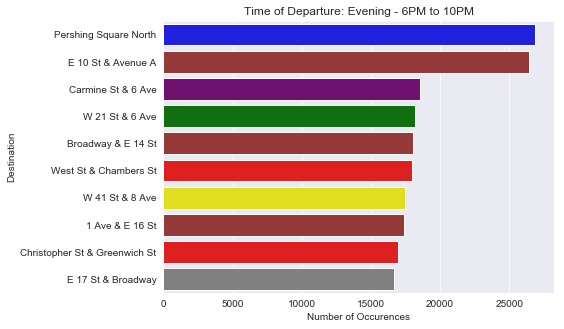
\includegraphics[scale = 0.6]{nightData} $$
Pershing Square North is still a very popular destination! This can be attributed to people leaving work and wanting to get on to the crowded trains at Grand Central Terminal, Apart from the usual Midtown locations, there are more stations that was popular in this time frame in other areas. East $10$th Street and Avenue A was the second most popular destination followed by Carmine St and $6$th Avenue. These two stations are located in the villages (East/West Villages, for those who are not familiar with NYC terminology). E $10$th Street and Avenue A is on the corner of Tompkins Square Park, which many people might be doing to for park activities. Carmine St and $6$th Avenue is located in West Village, a lively neighborhood with many bars and restaurants. Hence it should be of no surprise that bikers at this hour are going here. \\~\\
 For the late night bikers from $10$PM to $5$AM: 
$$ 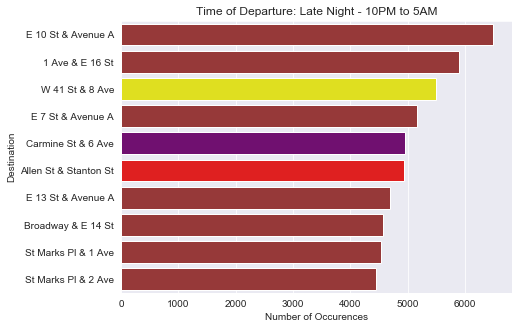
\includegraphics[scale = 0.6]{latenightData} $$ 
Pershing Square North is finally gone. It seems like people are not going to or leaving to work in Midtown at this time. Of the top $10$ destinations found, $7$ of them are East Village and $1$ is West Village. As popular youth neighborhoods, people may be traveling to this places at these hours for parties and other various activities. Do note that the $10$th most popular destination for the previous time frame had a count of over $15,000$ which the top most in this time frame has $6,000$. Therefore this does not mean that Citi bikes were just as frequently used. It can be seen that bike rides are of lesser quantity, probably because everyone is sleeping. But as they say, NYC is the city that never sleeps; therefore people are always up at all hours, as can be seen in the villages from $10$PM to $5$AM. \\~\\

This type of data is important to analyze because information of which places are popular at which hours and so where would most Citi bikes be located at which hours. This can help facilitate with the maintenance of bikes. It would be tragic if someone at Pershing Square North couldn't find a bike to ride while also being in a huge populated area. \newpage

\section{Distribution of User Types by Age}
The second question that was answered was, what is the distribution of user types by age. It is important to note that before querying the data, many records were removed so that it does not interfere as noise, such as users who were using the bike for at least $10$ days (I think those bikes were just stolen at that point or trashed) and users who are older than $65$. I do not believe we have a large number of elderly people trying to navigate through NYC with a bike. Coming back to the question, this was the distribution found: 
$$ 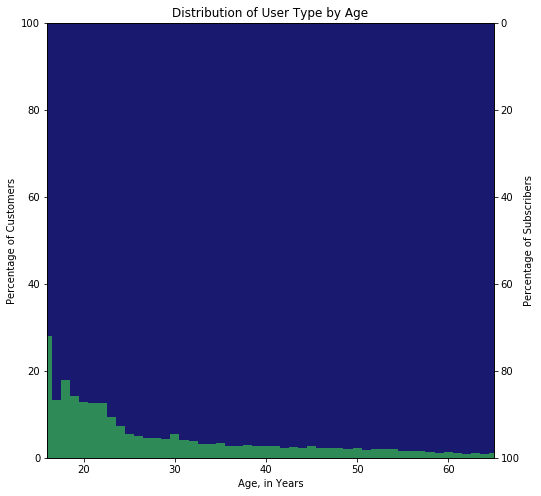
\includegraphics[scale = 0.7]{userTypeAge} $$ \newpage
As seen in this plot, short term customers were people in their $20$s and $30$s. After approaching $40$, the percentage of customers levels off to less than $5\%$. There are several reasons for why this could happen. First, the number of bikers increases from $16$ to $30$ and then start decreasing. This continues indefinitely up to $65$. This can be seen in the plot above. If there are more people riding Citi bike, then there is a more likelihood that more people could be a customer or subscriber. Now, in this age range, people are active; people want to be active. Therefore they are likely to do activities that require physical strength and health. Biking in NYC is one of those things and so people turn to this for their mode of transportation so they can be somewhat active. It is likely that more people are customers because they may be attempting to try using a bike first before thinking about depositing money on an annual membership. Note also that the highest percentage of customers is at age $16$, an age where people are still in high school and most likely getting free MTA metrocards. Therefore, buying a $\$169$ membership card may seem out of logic for the time being and so these kids are more likely to buy day passes whenever needed. 
People in their $20$s and $30$s are also more likely to be customers who used a bike as a last minute choice for transportation or could be just young tourists. \\~\\

This type of data is important to analyze because it shows which age groups have more customers than subscribers. By using this information, one can made advertisements targeting customers who may be paying more per ride than by getting an annual membership. 
\newpage
\section{Distribution of Bike Uses depending on time of Day, type of Day and Gender}
The third question that was answered was, what is the distribution of the number of bikes leaving and arriving based upon the hour, gender and type of day. The type of day was divided into two, where one group is weekdays and the other group is weekends. First the distribution for weekday is shown. \\~\\
The distribution of men riding a bike on a weekday is as follows: 
$$ 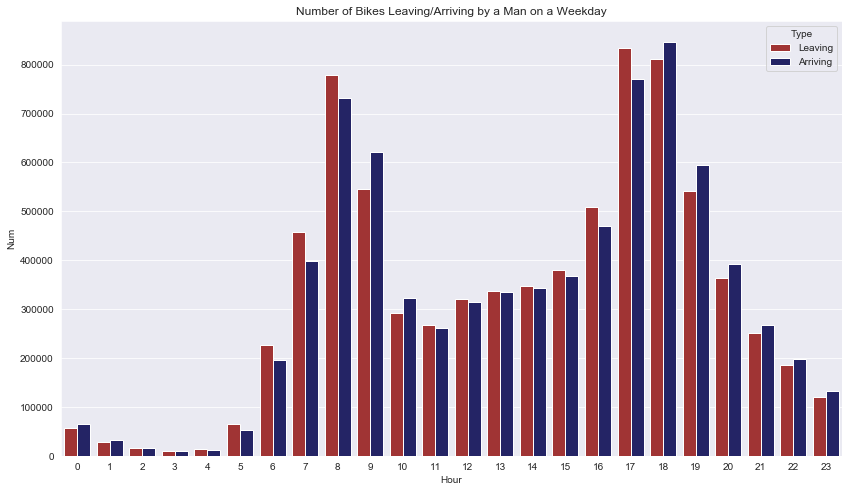
\includegraphics[width = \textwidth]{maleWeekday} $$ 
This distribution is bimodal, which would make sense. On weekdays, there are more people who are going to work and have work hours. Therefore seeing a high number of bike rides around $7$AM and $6$PM should be of no surprise. Bike rides come to an absolute low at around $3$AM, which is when many people are sleeping. Apart from the timing of the bike rides, the type of the bike ride was also noted. Despite making this separation, it can be seem that whether a bike is leaving or arriving at a station, it follows the same distribution. There are highs during rush hours and lows during night hours. There's a high number of arriving bikes at $8$AM and $9$AM which is due to the people who left at $7$AM and $8$AM for work. In fact, the number of bikes arriving at $9$AM and $6$ outnumber the number of bikes leaving at that time. Between these two high points, bike rides tend to decrease up to $11$AM and then starts picking up to $6$PM and then decrease til $3$AM. The low points occur at $2$AM to $4$AM. In fact, the proportion of bike trips at low hours to high hours is around $6\%$. This is a huge difference. 
\\~\\

The distribution of women riding a bike on a weekday is as follows: 
$$ 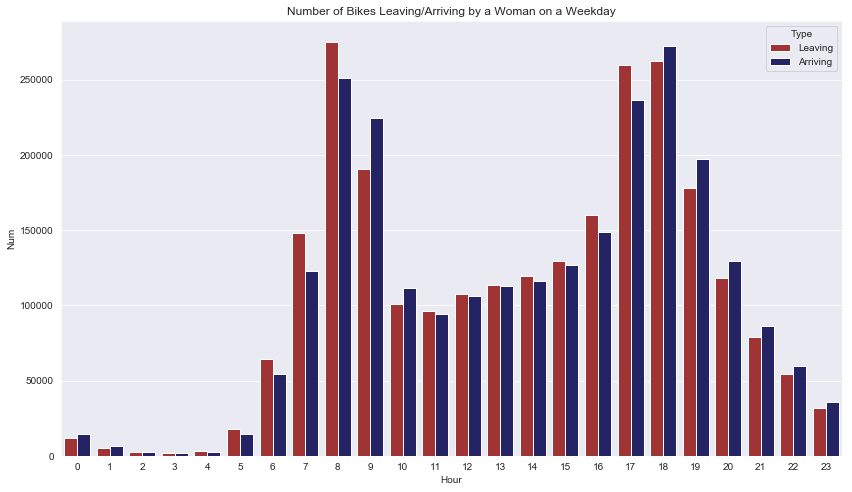
\includegraphics[width = \textwidth]{femaleWeekday} $$ 
A similar pattern is noticed with women on a weekday. Many of them are working and so there is a high point around $7$AM and $5-6$PM. In addition, we note that the high points have number of bikes rides at slightly above $250,000$. Looking back at the previous plot, the high points of occurrences of men at rush hours were in the ball park of $800,000$. This is $3$ times as much as the female counterpart. Similar to men, bike rides from midnight to $4$AM dip to an absolute low and then resume. The proportion of bikers at low hours to high hours is less than $10\%$. \\~\\

The distribution of men riding a bike on a weekend is as follows: 
$$ 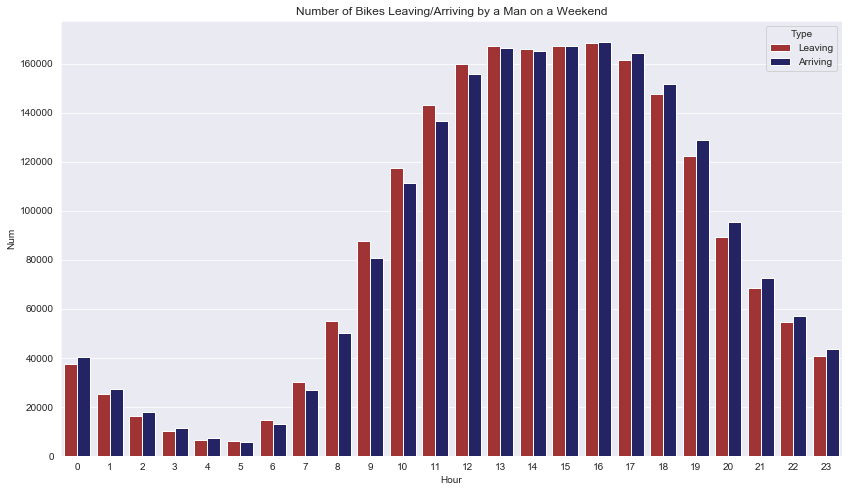
\includegraphics[width = \textwidth]{maleWeekend} $$ 
Unlike the previous distributions, this one follows a sinusoidal pattern and has only one high point and one low point. The greatest number of bike rides around $2$PM to $4$PM. This contrasts the weekday workflow schedule that many people have. It can be understood that people are riding bikes at these afternoon hours to enjoy the weather and free time. The number of bikes leaving from $5$AM to $2$PM overpasses the number of bikes arriving from $5$AM to $2$PM but then flips so that there are more bikes arriving than leaving from $2$PM to $5$AM. The highest count of bike ride for men on a weekday was $800,000$ which on a weekend it is slightly above $160,000$. This is a reduction of $80\%$ in the number of bike rides, generally speaking. The low points are at $4$AM and $5$ which makes sense because it is late night. But because it is the weekend and people are often out late night, it should be no surprise that there are bikers out from midnight to $2$AM. For the weekend, there are between $20,000$ to $40,000$ bike visits which is just $25\%$ of the ones at $4$PM. \\~\\

The distribution of women riding a bike on a weekend is as follows: 
$$ 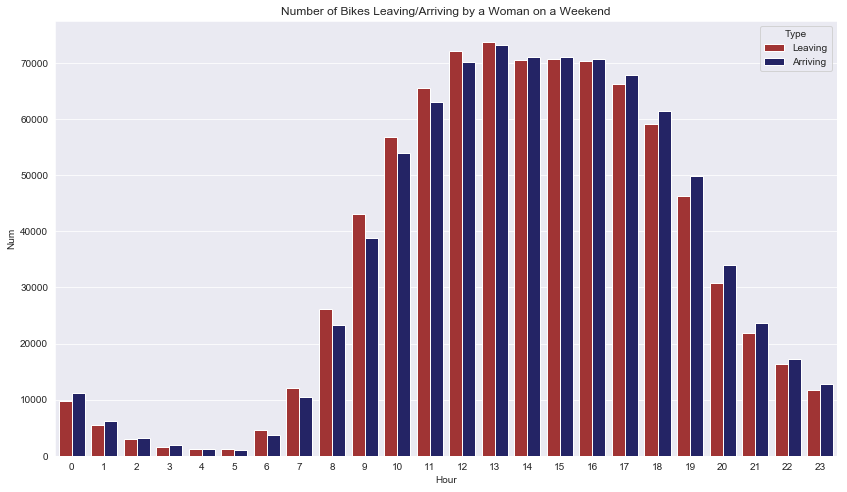
\includegraphics[width = \textwidth]{femaleWeekend} $$ 
This follows the same trend as the previous distribution. It is shaped with a sinusoidal pattern with highs around $2$PM to $3$PM and lows at $3$AM to $5$AM. The high point have at least $70,000$ bike trips which at the lows it hovers around $1,000$ bike visits. This is basically an average of $10$ bike trips for weekend day. \\~\\

This type of data is important to analyze because it explains the bike traffic of different demographics depending on the type of day. One could also do a similar analysis but broken up by each day rather than weekday/weekend but for a general overview, I believe this already gives a lot of information. 
\newpage
\section{Most Used Bikes and Total Hours Used}
The fourth question that was answered was finding the top most used bikes, with respect to bother number of uses and total number of hours in use. For this analysis, no bike IDs were filtered out for any reason other than if the person's age fell outside $18$ and $65$, had an unknown gender or were on a prolong bike trip. \\~\\
The most commonly used bikes are shown below: 
$$ 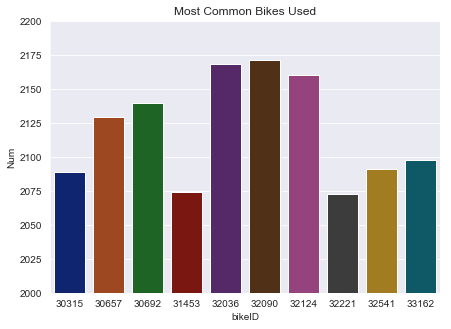
\includegraphics[width = \textwidth]{mostUsedBikes} $$ 
These bikes were amongst the $14,851$ distinct bikes that were most used. Three bikes were were used more than $2150$ times in the ten month of this dataset. This could mean that on average, these bikes were used at least $7$ times in a day. That's a lot considering that are thousands are bikes that can be used. For additional information, another query were made to find how many distinct bikes were rode less than $5$ times and how many were rode more than $1500$ times. What was found was that $42$ bikes were rode less than $5$ times while $5104$ bikes were rode more than $1500$ times. \\~\\

This information is valuable because it would tell which bikes are at risk of being damaged and/or need to be repaired. Further investigation can also be done that tracks each of these bikes to see if it is being heavily ridden for longer times. \\~\\
The distribution for most hours used bike are shown below: 
$$ 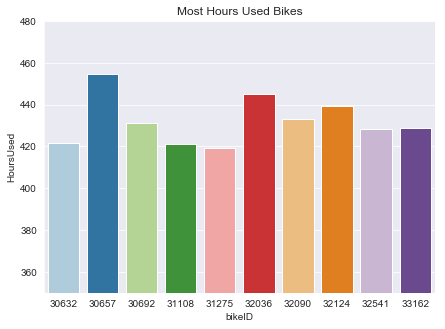
\includegraphics[width = \textwidth]{mostHoursUsedBikes} $$ 
This bar graph shows that ten bikes were used for more than $420$ hours in 2018. That is roughly $1.4$ hours per day, or $3$ or $4$ times in a day, on average. Bike number $39657$ was used the longest, at nearly $460$ hours. Comparing this plot with the above plot, bike number $30657$, $30692$, $32036$, $32090$, $32124$, $32541$ and $33162$ were amongst the top used bikes with respect to number of times and number of hours used. 
\\~\\
This information is valuable because it would also help which bikes may need to be looked at. As noted above, seven bikes were found from amongst the top ten of both queries that may need to get serviced. Further investigation could go into bikes that are least used so those can get more attention. As stated before, several bikes were found that were rode less than $5$ times in $10$ months. This could mean a problem with the bike itself, or someone may be hoarding it. 
\newpage
\section{Average Speed Traveled and Average Distance by Gender and Age}
The fifth question that was answered was finding the distribution of average speed traveled and average distance traveled by gender and age. This type of information can be used for studies on peoples' general health in NYC. In the dataset, distance traveled is not given but the coordinates of the start and end stations are given. Using this, the distance traveled during a trip ride is calculated using the haversine formula. This formula is used to determine the great-circle distance between two points on a sphere given their longitudes and latitudes. \\
Let $\phi_1$, $\phi_2$ represent the latitude of point 1 and latitude of point 2, respectively. Let $\lambda_1$, $\lambda_2$ represent the longitude of point 1 and longitude of point 2. Then the distance between the two points is
$$ d = 2r\arcsin \left( \sqrt{ \sin^2 \left( \frac{\phi_2 - \phi_1}{2} \right) + \cos(\phi_1)\cos(\phi_2)\sin^2\left( \frac{\lambda_2 - \lambda_1}{2}\right)} \right) $$
where $r$ is the the radius of the sphere. In our case, it is the radius of Earth. Using this, the average distance and average speed was computable. \\~\\ 
The average speed is shown below: 
$$ 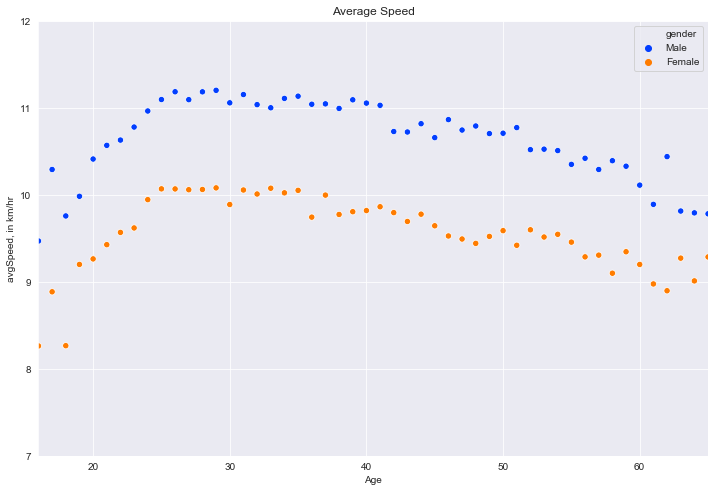
\includegraphics[width = \textwidth]{avgSpeed} $$ 
There are some similarity between the average speed of men and women. What's similar between them is the general direction of the curve. From the age of $16$ to mid/late $20$s, men and women both tend to be faster at biking. The difference in average speed come out to an estimated $2.5$ kilometers/hour for men from the age of $18$ to $28$ while for women it is $2$ kilometers/hour. After the late $20$s, people start to ride their bike slower. As for the differences, men tend to ride $1$ to $1.5$ kilometers/hour faster than women at any age. \\~\\
The average distance is shown below: 
$$ 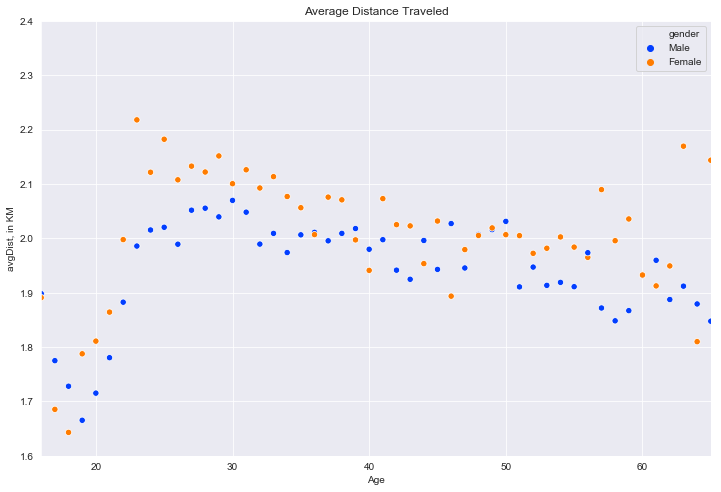
\includegraphics[width = \textwidth]{avgDist} $$ 
Just like with average speed, men and women tend to follow similar patterns in how much they bike. People as young as $16$ have an average distance of $1.7$ kilometers which then picks up to $2.1$ kilometers for people in their mid $20$s. The average distance traveled then starts to fall all the way down to $1.8$ kilometers. What's different in this analysis is that despite women traveling slower than men on the average, women do tend to travel more distance than men. What this means is that one group has more endurance (higher average speed) which the other group can last longer (longer distance). This type of information is valuable because it shows how age affects how much one can/is willing to travel by bike. Younger people travel less than people in their $20$ but then start falling, maybe due to old age.

The maximum distance traveled by a single person per age is also plotted just to see if there is any pattern. 

$$ 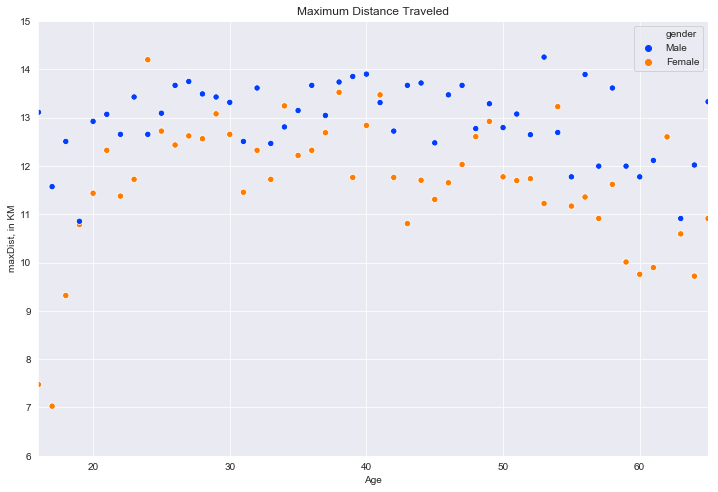
\includegraphics[width = \textwidth]{maxDist} $$ 
It is a general pattern that there is 1 man who will have biked a longer distance than the longest female biker. Their differences tend to be in the range of $1$ to $2$ kilometers. This form of statistic can be used in campaigns to get more female bicyclers in races to compete against men. 
\newpage
\section{Linear Regression Model} 
As an added bonus, a linear regression model was created that predicted the time it would take to go from one station to another. A linear regression model was ran through the entire dataset of $13$ million observations This was the result: 
$$ 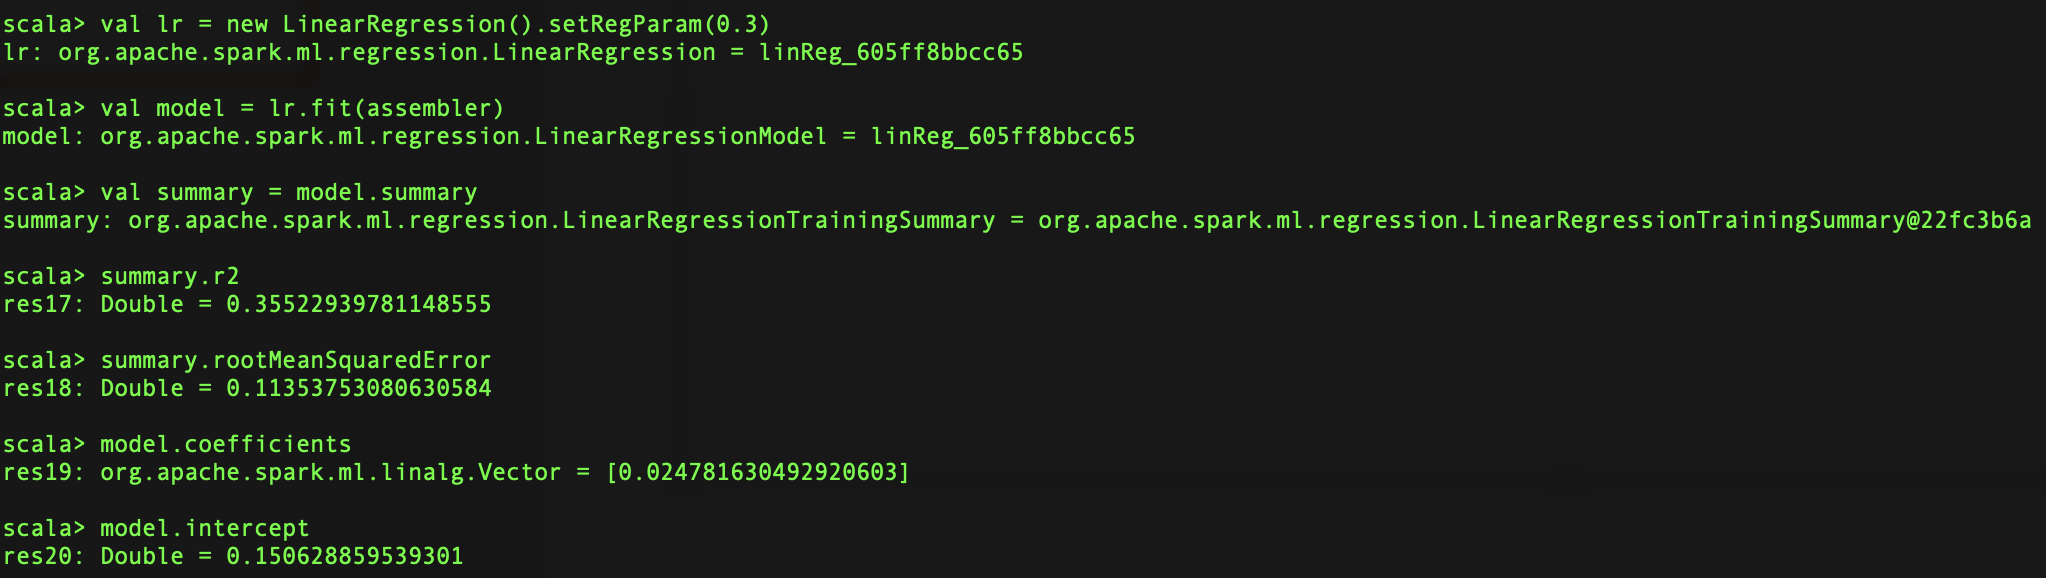
\includegraphics[width = \textwidth]{model} $$ 
The model has a $R^2$ value of $0.35$ and an RMSE of $0.11$. In mathematical context, the RMSE is the square root of the variance of the residuals. It tells in mathematical terms how close the data points are to the model's predicted values. It can be interpreted as the standard deviation of the unexplained variance. Since the RMSE value calculated from the model is not too high, the model is a decent fit for the data. With the values determined by the regression algorithm, the equation to determine the time a biker will take to travel from station to another is
$$ y = 0.1506 + 0.0247x $$ where $x$ is the distance between the station, in kilometers, and $y$ is the time in hours. \\
However the $R^2$ value could improve. Building the model on other features such as age, user type, etc could make the model better. The distance that was used in this model creation was a simple computation of the distance between two station. it may be that if two different routes, with different start and end stations, have the same distance between them, the time should also represent this differentiation. This would require more work to be done. Other features such as month of bike ride and weather may also affect the trip duration of a bike ride. What could also be a false indicator is the fact that the Haversine formula was used to calculate the distance between two points. Looking at a linear algebra point of view, it gives the shortest distance between two points. In the real world case, that is likely not true; one does not navigate through NYC in a straight line but by taking turns here and there. Therefore actual distance traveled could be greater. 

\newpage
\section{Conclusion} 
Though out this project, several analyses were mined from the Citibike dataset of $10$ months of data. This dataset was large, $2.7$ gigabytes, and could not be handled using Microsoft Excel. Therefore trying to analyze data in Spark using RDDs to do parallel computations was easier. It managed to handle millions of observations and find answers to several questions. It can be seen that certain neighborhoods are popular destinations at different hours, such as Midtown East in the morning and East/West Village late night. Young bikers are more likely to be short term customers than annual subscribers. Bike traffic for men and women do not differ by time but similar patterns are found when comparing if they bike in the weekend or weekday. Most used bikes were found that can help mechanics try to find bikes that may need servicing due to long usage. It was also found that men had a higher average speed on a Citi Bike than women for all ages while the opposite was observed in the average distance traveled. The questions answered here are not extensive and more can always be answered. In addition, the linear regression returned some unfavorable results when predicting trip duration from distance. It would be suggested to add more features to the linear regression model and play with the hyper parameters. 

\end{document} 